%% LyX 2.3.2 created this file.  For more info, see http://www.lyx.org/.
%% Do not edit unless you really know what you are doing.
\documentclass[english]{article}
\usepackage[T1]{fontenc}
\usepackage[latin9]{inputenc}
\usepackage{geometry}
\geometry{verbose,tmargin=2cm,bmargin=2cm,lmargin=2cm,rmargin=2cm}
\PassOptionsToPackage{natbib=true}{biblatex}
\usepackage{float}
\usepackage{textcomp}
\usepackage{amstext}
\usepackage{graphicx}

\makeatletter

%%%%%%%%%%%%%%%%%%%%%%%%%%%%%% LyX specific LaTeX commands.
\newcommand{\lyxmathsym}[1]{\ifmmode\begingroup\def\b@ld{bold}
  \text{\ifx\math@version\b@ld\bfseries\fi#1}\endgroup\else#1\fi}

%% Because html converters don't know tabularnewline
\providecommand{\tabularnewline}{\\}

%%%%%%%%%%%%%%%%%%%%%%%%%%%%%% User specified LaTeX commands.
\usepackage{ae,aecompl}

\makeatother

\usepackage{babel}
\usepackage[style=trad-unsrt,backend=bibtex8]{biblatex}
\addbibresource{phytoInteractions_ref.bib}
\addbibresource{bib_fig_review.bib}
\begin{document}
\emph{Supplementary Information} for \textbf{Strong self-regulation
and widespread facilitative interactions between groups of phytoplankton
}- Picoche, C. \& Barraquand F.


\appendix
\begin{figure}[H]
\begin{centering}
\includegraphics[width=0.99\textwidth]{graphe/placing_points_gnom}
\par\end{centering}
\caption{\textbf{Location of each study site in their region}: Brittany (A),
Ol�ron (B), Arcachon (C) and the Mediterranean Sea (D). The common
scale of the panels in given in the left corner of D. \label{fig:Map}}
\end{figure}

\begin{table}[H]
\begin{centering}
\begin{tabular}{cc}
\hline 
\textbf{Code} & \textbf{Taxa}\tabularnewline
\hline 
AST & Asterionella+Asterionellopsis+Asteroplanus\tabularnewline
CHA & Chaetoceros\tabularnewline
CRY & Cryptophytes\tabularnewline
DIT & Ditylum\tabularnewline
EUG & Euglenophytes\tabularnewline
GUI & Guinardia\tabularnewline
GYM & Gymnodinium+Gyrodinium\tabularnewline
LEP & Leptocylindrus\tabularnewline
NIT & Nitzschia+Hantzschia\tabularnewline
PLE & Pleurosigma+Gyrosigma\tabularnewline
PRO & Prorocentrum\tabularnewline
PRP & Protoperidinium+Archaeperidinium+Peridinium\tabularnewline
PSE & Pseudo-nitzschia\tabularnewline
RHI & Rhizosolenia+Neocalyptrella\tabularnewline
SCR & Scrippsiella+Ensiculifera+Pentapharsodinium+Bysmatrum\tabularnewline
SKE & Skeletonema\tabularnewline
THL & Thalassionema+Lioloma\tabularnewline
THP & Thalassiosira+Porosira\tabularnewline
\end{tabular}
\par\end{centering}
\caption{\textbf{Name and composition of the phytoplanktonic groups used in
the paper}, based on \supercite{hernandez_farinas_assessing_2015}\label{tab:Group_definition}}

\end{table}

\begin{table}[H]
\begin{centering}
\begin{tabular}{cccccc}
\hline 
\textbf{Name of site} & \textbf{Location} & \textbf{Region} & \textbf{N. samples} & \textbf{Temperature (�C)} & \textbf{Salinity (g/L)}\tabularnewline
\hline 
Men Er Roue & 47�32' N / 3�5' W & Brittany & 503 & 14.4 +/- 3.7 & 33.5 +/- 1.9\tabularnewline
Loscolo & 47�27' N / 2�32' W & Brittany & 463 & 14.9 +/- 4.0 & 32.0 +/- 3.0\tabularnewline
Croisic & 47�18' N / 2�30' W & Brittany & 500 & 14.7 +/- 3.9 & 31.8 +/- 3.1\tabularnewline
L'Eperon & 46�16' N / 1�14' W & Ol�ron & 460 & 15.3 +/- 4.8 & 32.1 +/- 3.2\tabularnewline
Cornard & 46�3' N / 1�7' W & Ol�ron & 491 & 15.6 +/- 4.8 & 32.7 +/- 2.4\tabularnewline
Auger & 45�47' N / 1�12' W & Ol�ron & 524 & 15.4 +/- 4.4 & 32.7 +/- 1.8\tabularnewline
Buoy 7 & 44�32' N / 1�15' W & Arcachon & 311 & 15.2 +/- 3.8 & 34.7 +/- 0.7\tabularnewline
Teychan & 44�40' N / 1�9' W & Arcachon & 494 & 15.5 +/- 4.6 & 32.5 +/- 1.9\tabularnewline
Antoine & 43�22' N / 4�50' E & Mediterranean Sea & 539 & 16.8 +/- 5.1 & 32.3 +/- 3.9\tabularnewline
Lazaret & 43�5' N / 5�54' E & Mediterranean Sea & 512 & 17.4 +/- 4.2 & 35.9 +/- 2.4\tabularnewline
\end{tabular}
\par\end{centering}
\caption{\textbf{Summary of the study site characteristics}, including hhe
mean and standard deviation of the two main environmental parameters
(temperature and salinity). \label{tab:Site_description} }
\end{table}

\begin{figure}[H]
\begin{centering}
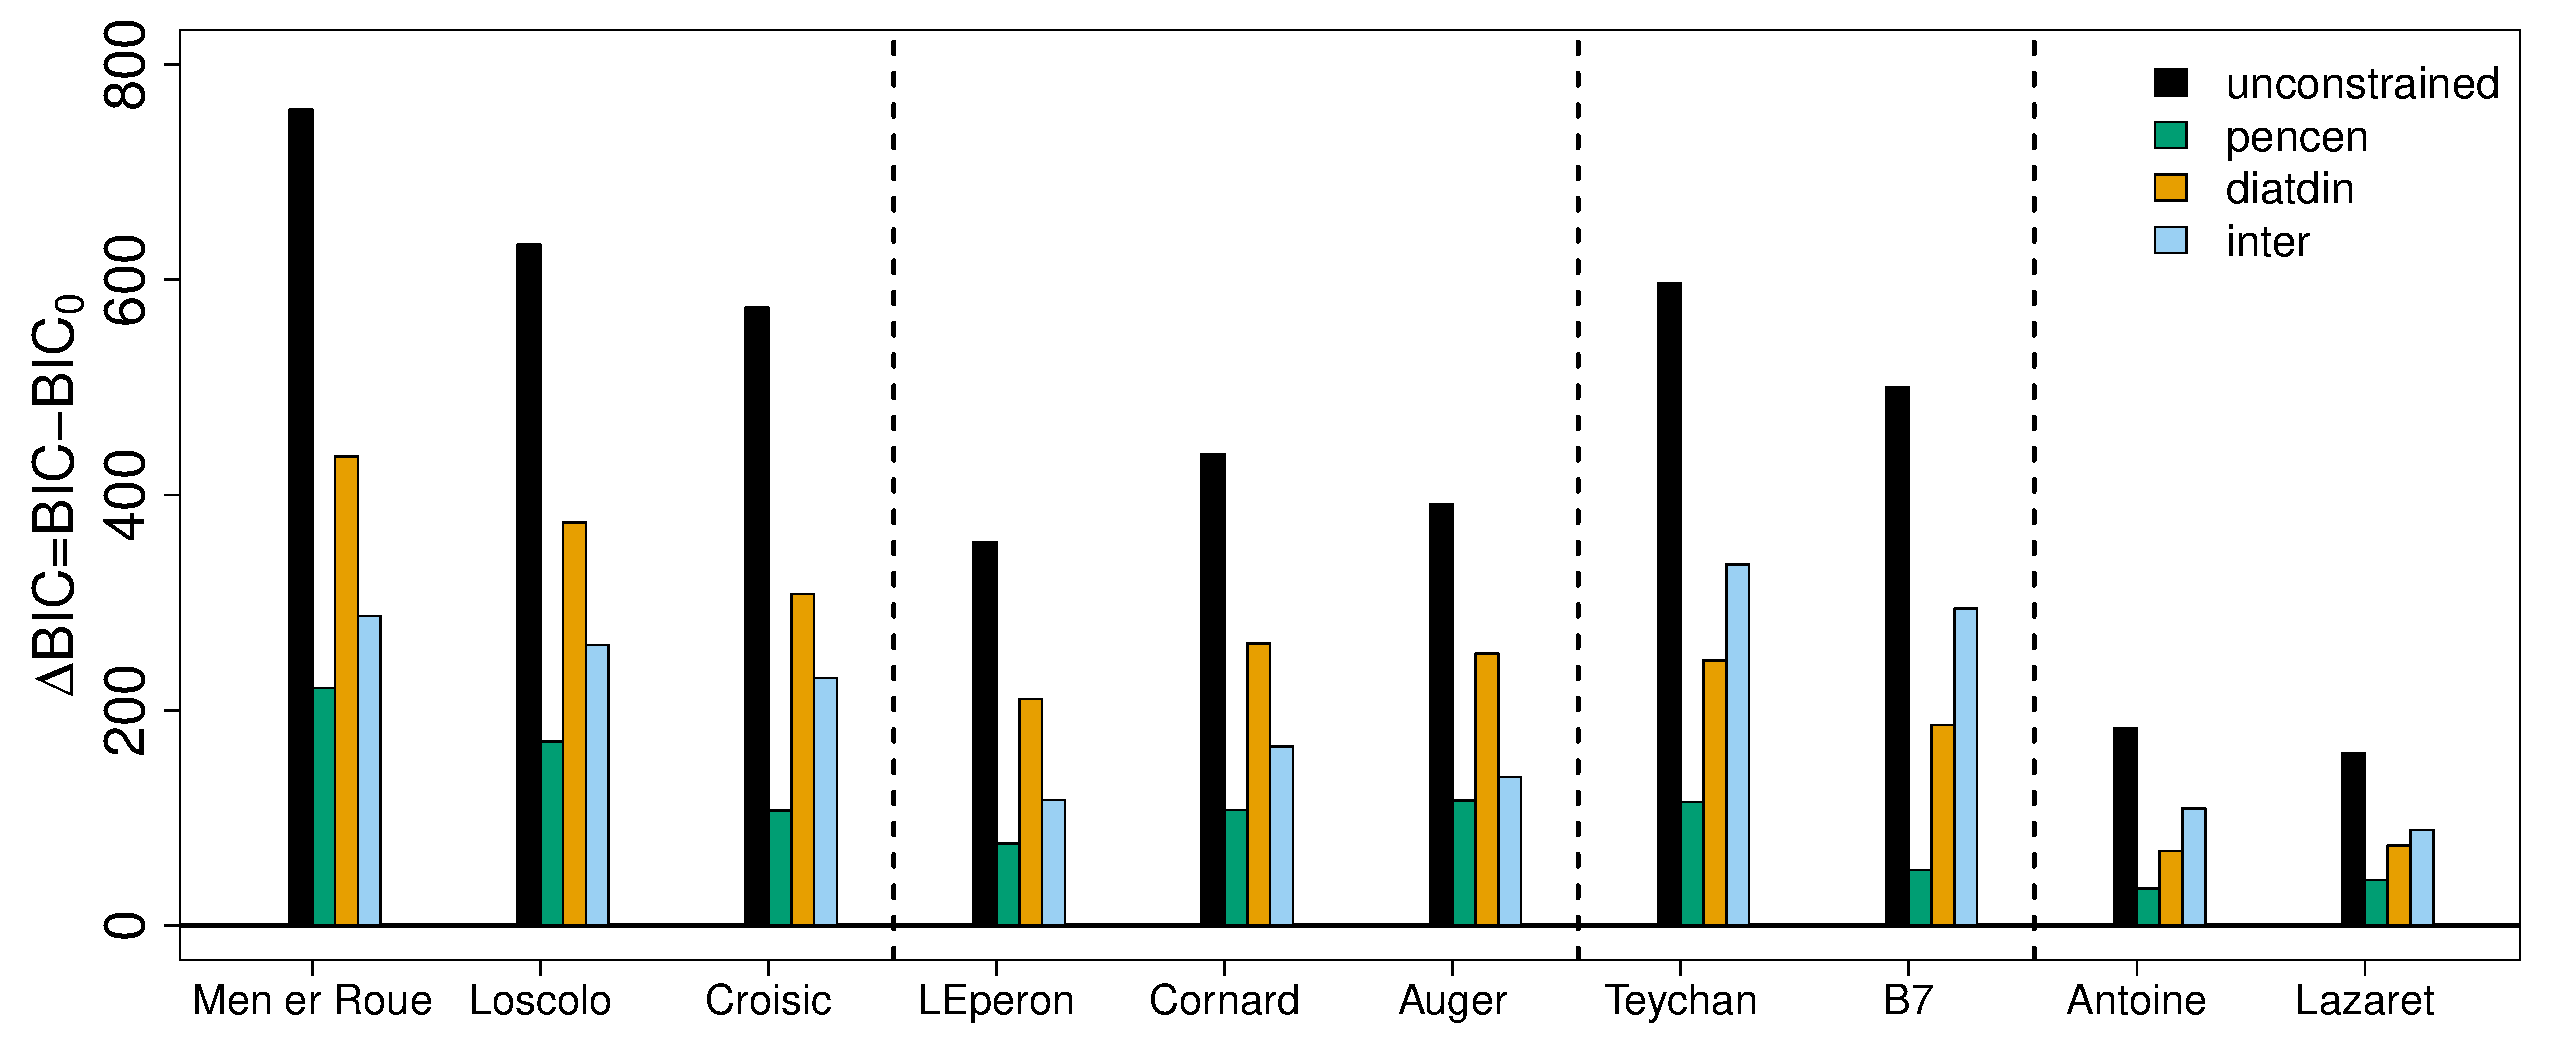
\includegraphics[width=0.99\textwidth]{graphe/comp_BIC_per_site}
\par\end{centering}
\caption{\textbf{Comparison of the BIC of different interaction models}, compared
to the null model (diagonal interaction matrix, allowing only intragroup
interactions), for 10 sites in 4 different regions, separated by dashed
lines (Brittany, Ol�ron, Arcachon and the Mediterranean Sea). Different
interaction matrices may allow interactions between all taxa (unconstrained),
only interactions within pennate diatoms, centric diatoms, dinoflagellates,
or other phytoplanktonic taxa (pencen), only interactions within diatoms,
dinoflagellates or other taxa (diatdin), or only interactions between
taxa belonging to these different groups. As model structures (length
of the times series taken into account) are different between sites
and regions, groups of bars should not be compared.\label{fig:Comparison-of-BIC}}
\end{figure}

\begin{figure}[H]
\begin{centering}
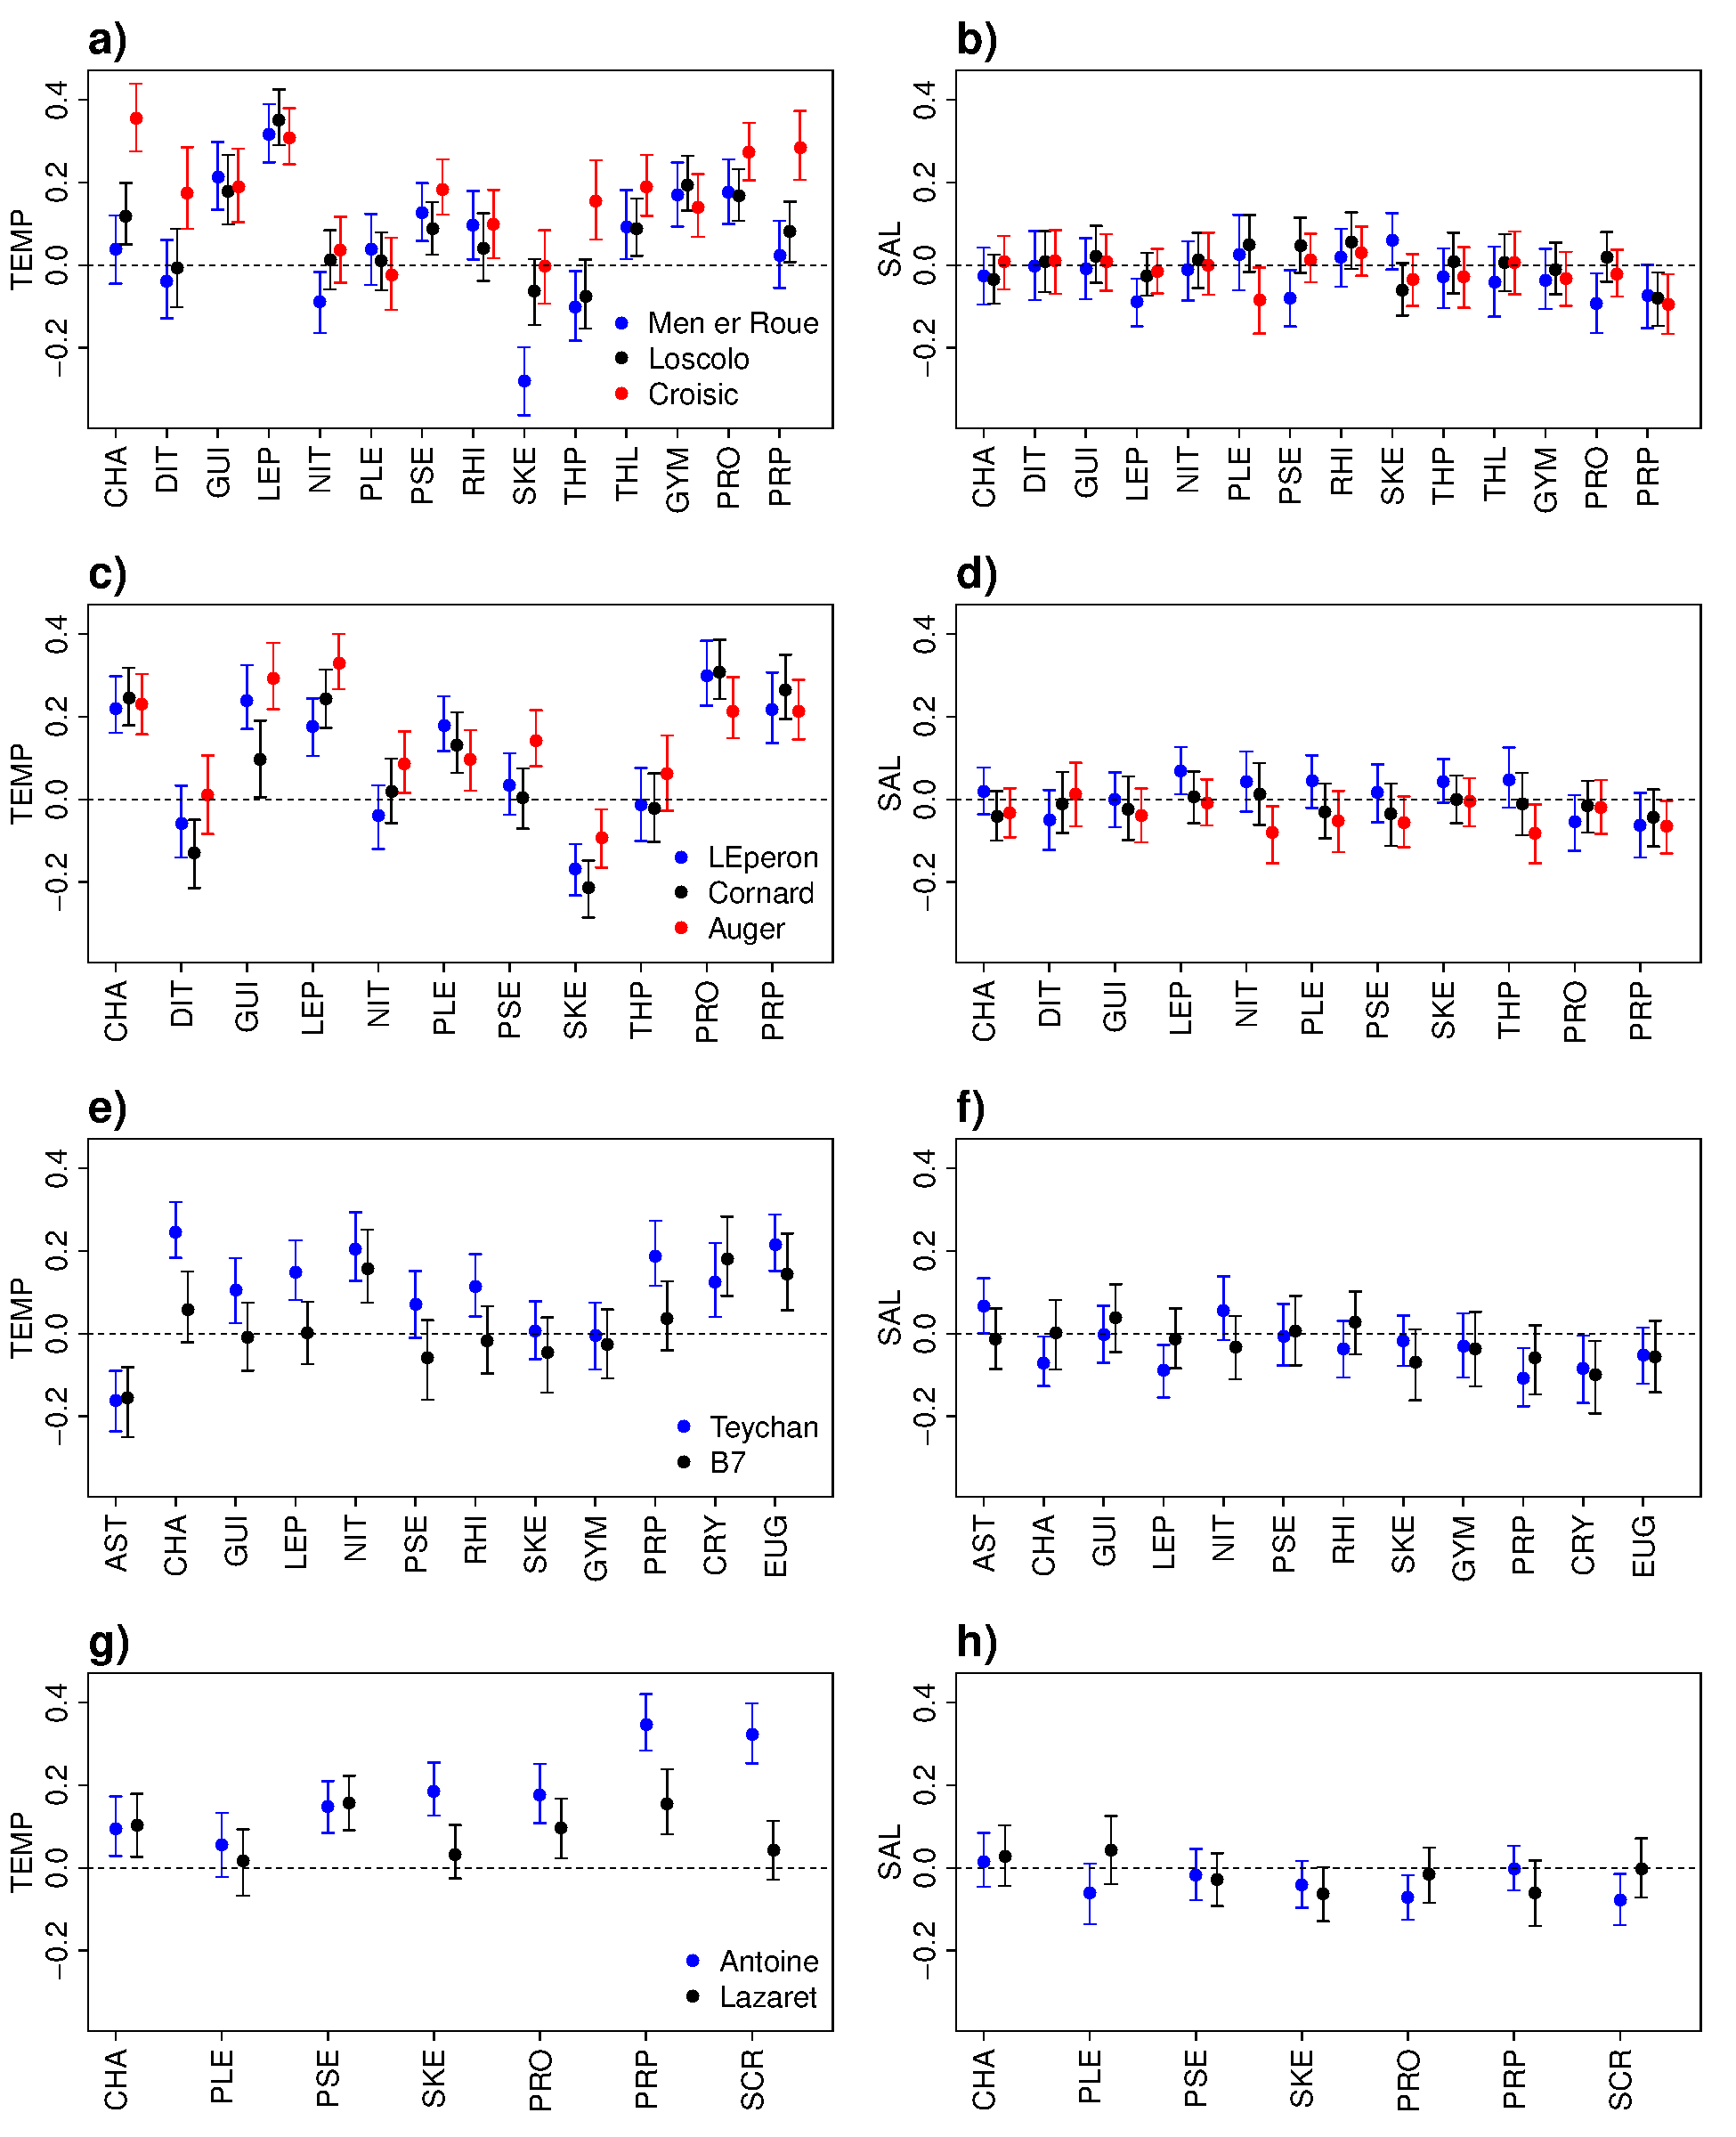
\includegraphics[width=0.99\textwidth]{graphe/abiotic_second_try}
\par\end{centering}
\caption{\textbf{Effect of environmental variables (temperature, TEMP or salinity,
SAL) on phytoplankton group} in Brittany (a, b), Ol�ron (c, d), Arcachon
(e, f) and in the Mediterranean Sea (g, h). Each color corresponds
to a different site. Error bars correspond to the 95\% confidence
interval around the estimated coefficient. All variables were normalized
before estimation. \label{fig:Abiotic_effects}}

\end{figure}

\begin{figure}[H]
\begin{centering}
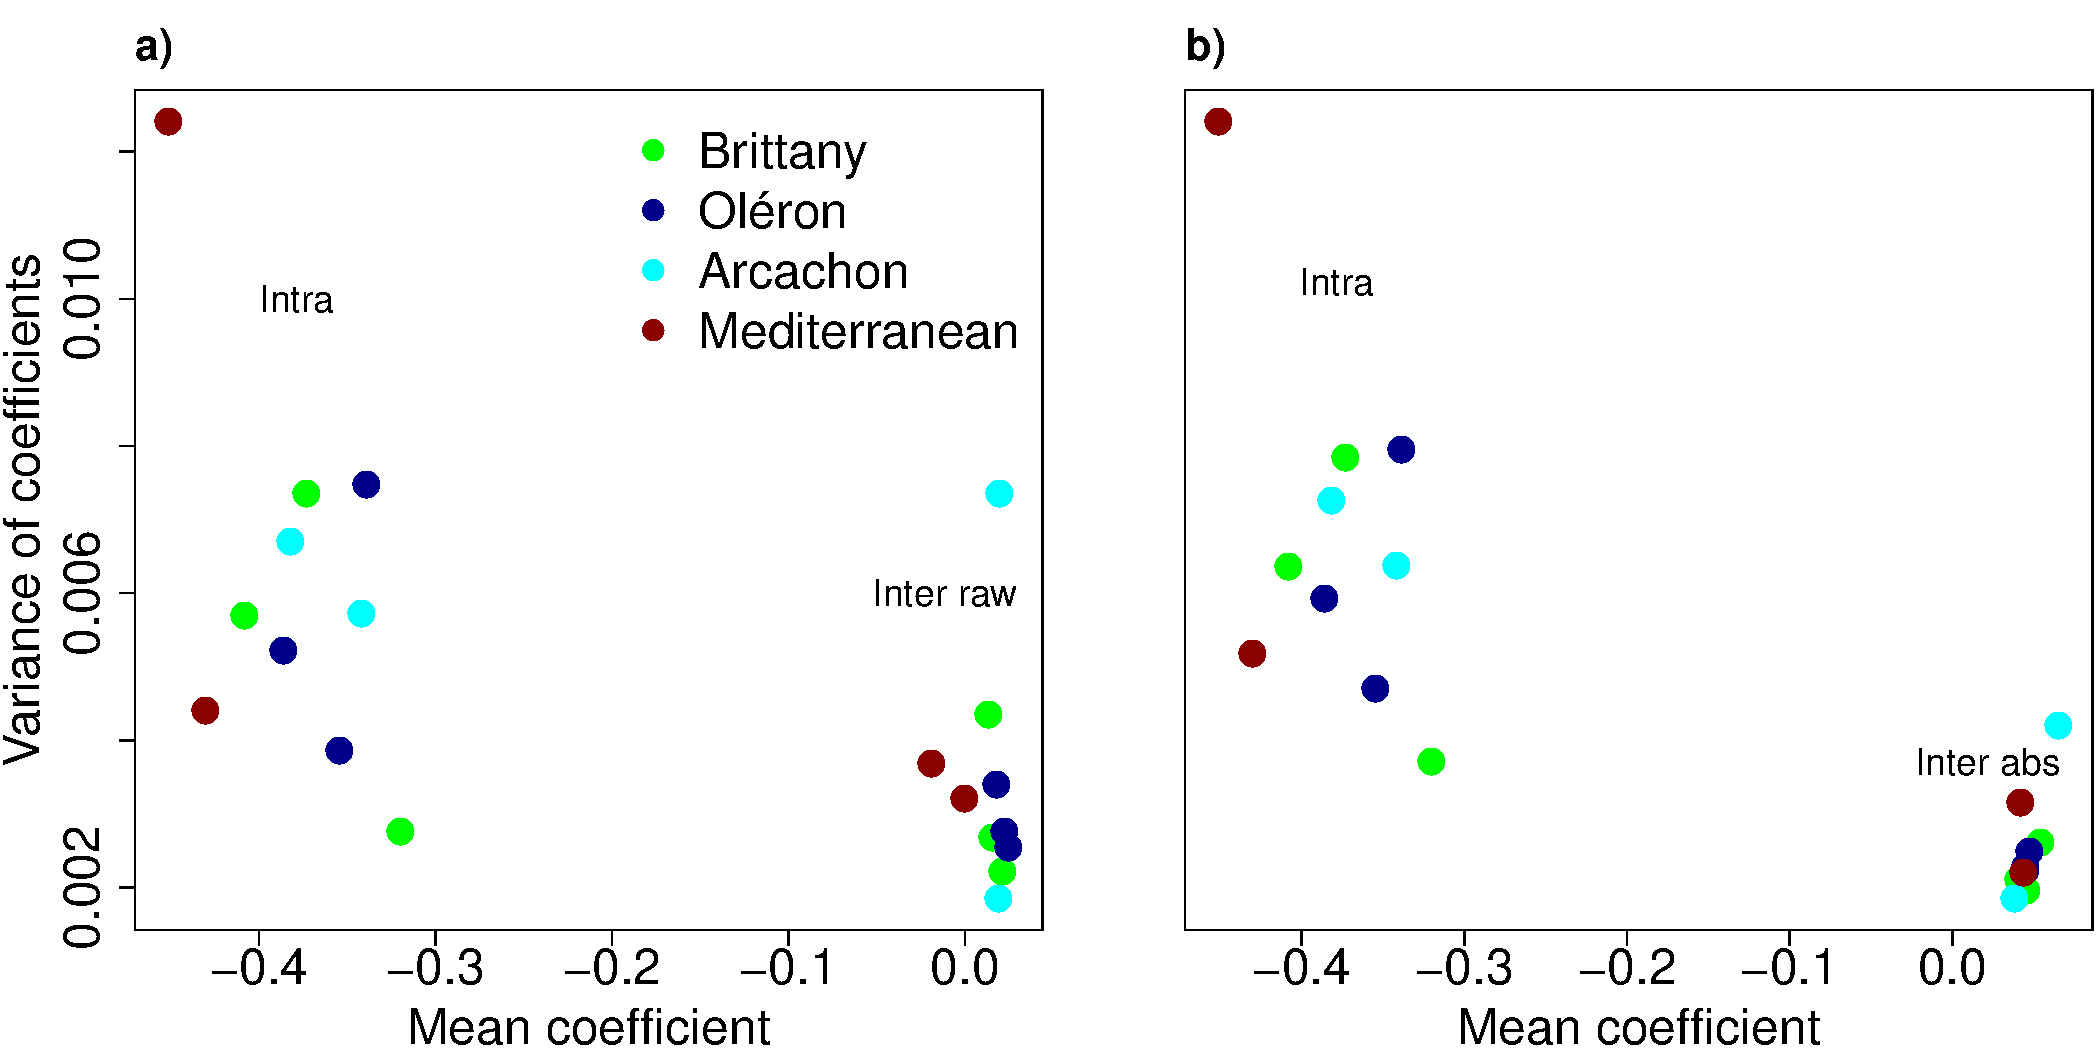
\includegraphics[width=0.99\textwidth]{graphe/moy_vs_var_for_all_interactions_pencen_SI}
\par\end{centering}
\caption{\textbf{Relation between mean and variance of the intra- and inter-group
interaction coefficients}. Variance of the coefficient in the interaction
matrix $(\mathbf{B}\lyxmathsym{\textendash}\textbf{I})$ is a function
of their mean, for 10 sites in 4 regions, with a model allowing interactions
only within clads (within centric or pennate diatoms, dinoflagellates,
or other taxa). The mean-variance relation was either computed with
raw values of intergroup interactions (a) or absolute values of the
intergroup coefficients (b). Intragroup coefficients were not modified.
\label{fig:MeanVar}}
\end{figure}


\subsection*{References for the meta-analysis}

\begin{table}[H]
\begin{centering}
{\footnotesize{}}%
\begin{tabular}{cccccc}
\hline 
\textbf{\footnotesize{}Code on the plot} & \textbf{\footnotesize{}Ref} & \textbf{\footnotesize{}Dimension} & \textbf{\footnotesize{}Type of organisms} & \textbf{\footnotesize{}System} & \textbf{\footnotesize{}T}\tabularnewline
\hline 
{\footnotesize{}1a} & {\footnotesize{}\citep{ives_community_1999}, CLS} & {\footnotesize{}9} & {\footnotesize{}Zooplankton} & {\footnotesize{}Lake} & {\footnotesize{}100}\tabularnewline
{\footnotesize{}1b} & {\footnotesize{}\citep{ives_community_1999}, TLS} & {\footnotesize{}9} & {\footnotesize{}Zooplankton} & {\footnotesize{}Lake} & {\footnotesize{}100}\tabularnewline
{\footnotesize{}2a} & {\footnotesize{}\citep{klug_compensatory_2000}} & {\footnotesize{}2} & {\footnotesize{}Phytoplankton} & {\footnotesize{}Lake} & {\footnotesize{}100}\tabularnewline
{\footnotesize{}2b} & {\footnotesize{}\citep{klug_compensatory_2000}} & {\footnotesize{}3} & {\footnotesize{}Zooplankton} & {\footnotesize{}Lake} & {\footnotesize{}50}\tabularnewline
{\footnotesize{}3a} & {\footnotesize{}\citep{klug_interactions_2001}} & {\footnotesize{}4} & {\footnotesize{}Functional groups of plankton} & {\footnotesize{}Lake} & {\footnotesize{}300}\tabularnewline
{\footnotesize{}3b} & {\footnotesize{}\citep{klug_interactions_2001}} & {\footnotesize{}5} & {\footnotesize{}Taxonomic groups of plankton} & {\footnotesize{}Lake} & {\footnotesize{}300}\tabularnewline
{\footnotesize{}4a} & {\footnotesize{}\citep{ives_estimating_2003}} & {\footnotesize{}4} & {\footnotesize{}Plankton} & {\footnotesize{}Lake} & {\footnotesize{}100}\tabularnewline
{\footnotesize{}4b} & {\footnotesize{}\citep{ives_estimating_2003}} & {\footnotesize{}4} & {\footnotesize{}Plankton} & {\footnotesize{}Lake with high planktivory} & {\footnotesize{}100}\tabularnewline
{\footnotesize{}4c} & {\footnotesize{}\citep{ives_estimating_2003}} & {\footnotesize{}4} & {\footnotesize{}Plankton} & {\footnotesize{}Lake with low planktivory} & {\footnotesize{}100}\tabularnewline
{\footnotesize{}5a} & {\footnotesize{}\citep{hampton_empirical_2006}} & {\footnotesize{}14} & {\footnotesize{}Plankton} & {\footnotesize{}Lake} & {\footnotesize{}300}\tabularnewline
{\footnotesize{}5b} & {\footnotesize{}\citep{hampton_empirical_2006}} & {\footnotesize{}14} & {\footnotesize{}Plankton, growing season} & {\footnotesize{}Lake} & {\footnotesize{}200}\tabularnewline
{\footnotesize{}6a} & {\footnotesize{}\citep{hampton_coalescence_2006}} & {\footnotesize{}13} & {\footnotesize{}Plankton} & {\footnotesize{}Lake} & {\footnotesize{}400}\tabularnewline
{\footnotesize{}6b} & {\footnotesize{}\citep{hampton_coalescence_2006}} & {\footnotesize{}7} & {\footnotesize{}Simpler web, plankton} & {\footnotesize{}Lake} & {\footnotesize{}400}\tabularnewline
{\footnotesize{}7a} & {\footnotesize{}\citep{huber_role_2006}} & {\footnotesize{}10} & {\footnotesize{}Ciliates} & {\footnotesize{}Lake} & {\footnotesize{}300}\tabularnewline
{\footnotesize{}7b} & {\footnotesize{}\citep{huber_role_2006}} & {\footnotesize{}10} & {\footnotesize{}Phytoplankton} & {\footnotesize{}Lake} & {\footnotesize{}300}\tabularnewline
{\footnotesize{}8a} & {\footnotesize{}\citep{yamamura_how_2006}} & {\footnotesize{}3} & {\footnotesize{}Insects} & {\footnotesize{}Terrestrial} & {\footnotesize{}50}\tabularnewline
{\footnotesize{}9a} & {\footnotesize{}\citep{vik_interlinking_2008}} & {\footnotesize{}2} & {\footnotesize{}Lynx/Hare} & {\footnotesize{}Terrestrial} & {\footnotesize{}100}\tabularnewline
{\footnotesize{}10a} & {\footnotesize{}\citep{lindegren_preventing_2009}} & {\footnotesize{}3} & {\footnotesize{}Fish} & {\footnotesize{}Baltic Sea} & {\footnotesize{}30}\tabularnewline
{\footnotesize{}11a} & {\footnotesize{}\citep{griffiths_phytoplankton_2015}} & {\footnotesize{}7} & {\footnotesize{}Phytoplankton} & {\footnotesize{}Coastal site} & {\footnotesize{}1000}\tabularnewline
{\footnotesize{}11b} & {\footnotesize{}\citep{griffiths_phytoplankton_2015}} & {\footnotesize{}7} & {\footnotesize{}Phytoplankton} & {\footnotesize{}Offshore site} & {\footnotesize{}700}\tabularnewline
{\footnotesize{}12a} & {\footnotesize{}\citep{barraquand_coastal_2018}} & {\footnotesize{}12} & {\footnotesize{}Phytoplankton} & {\footnotesize{}Outside a bay} & {\footnotesize{}300}\tabularnewline
{\footnotesize{}12b} & {\footnotesize{}\citep{barraquand_coastal_2018}} & {\footnotesize{}12} & {\footnotesize{}Phytoplankton} & {\footnotesize{}Inside a bay} & {\footnotesize{}500}\tabularnewline
\end{tabular}{\footnotesize\par}
\par\end{centering}
\caption{Studies used when comparing |intra|/|inter| ratios in Fig. 4 in main
text and Supplementary Fig. \ref{fig:Ratio-of-intra-to-intergroup}.
T is the approximate number of sampling dates in each time series.
\label{tab:Studies}}

\end{table}

\begin{figure}[H]
\begin{centering}
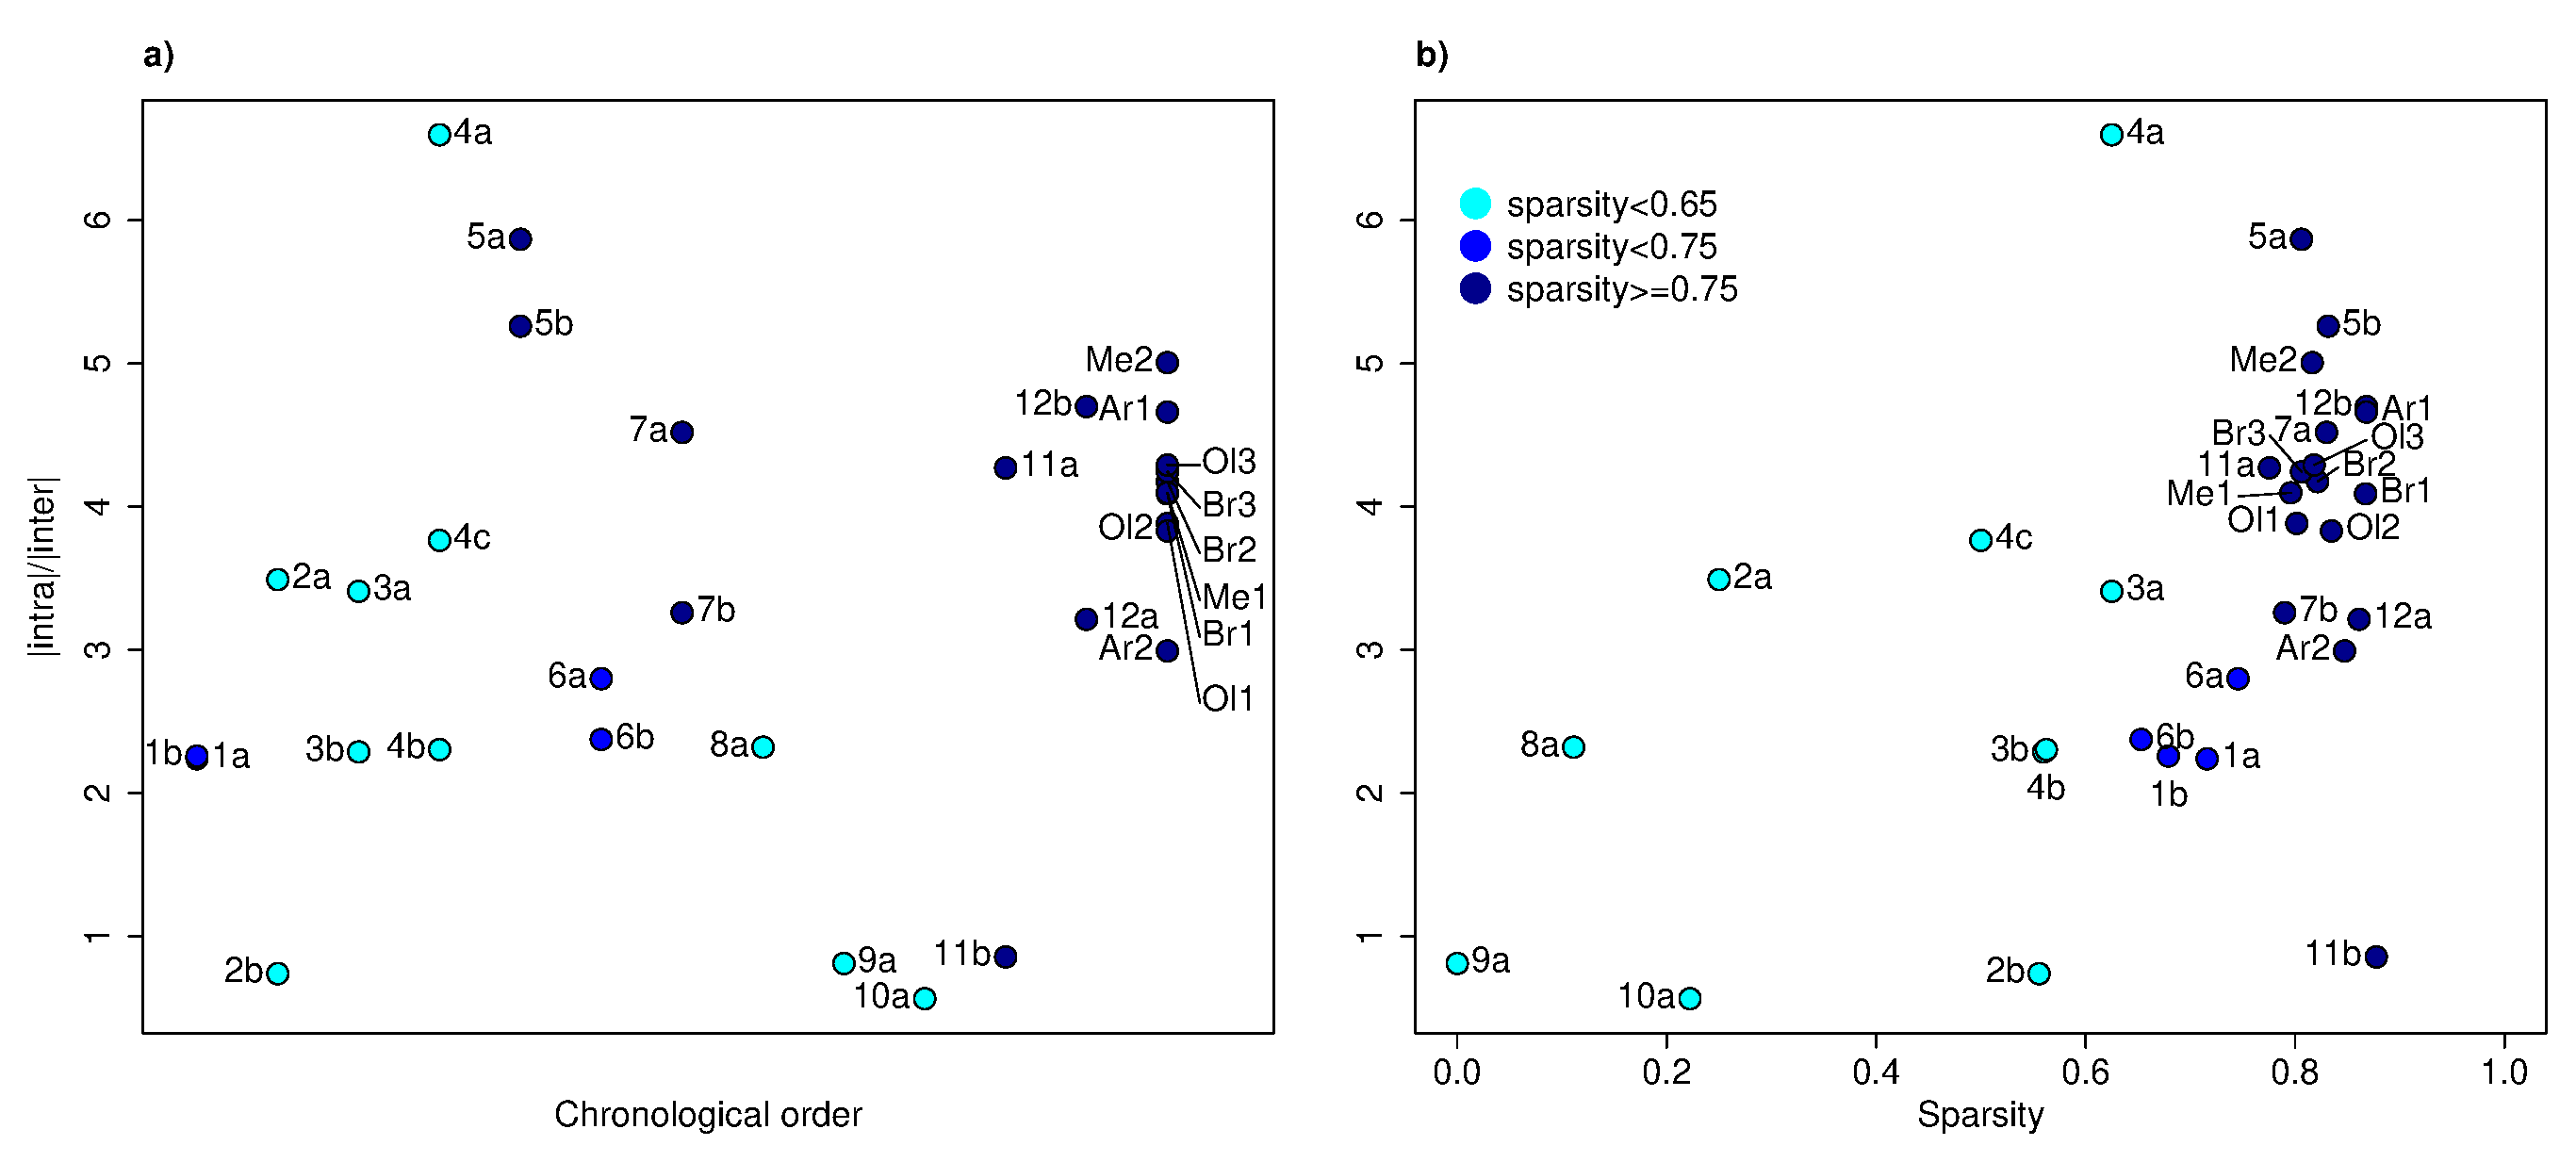
\includegraphics[width=0.8\textwidth]{graphe/comparaison_ratio_code_nolog_cleaner_ONLY_SIGNIF}
\par\end{centering}
\caption{\textbf{Ratio of intra-to-intergroup interaction strength in MAR(1)
studies. }Only significant values are taken into account and missing
values in the matrix are not considered (e.g., not replaced by 0 as
they are in the main text). The color of each point is a function
of the sparsity of the interaction matrix B-I and the relation between
the raio and the sparsity of the matrix is given in the right panel.
Corresponding studies are described in Table \ref{tab:Studies}. \label{fig:Ratio-of-intra-to-intergroup}\textit{
}\textbf{\textit{{[}This graph is not the final one but I'm wondering
if we keep it{]}}}\textit{ }}
\end{figure}

\begin{figure}[H]
\begin{centering}
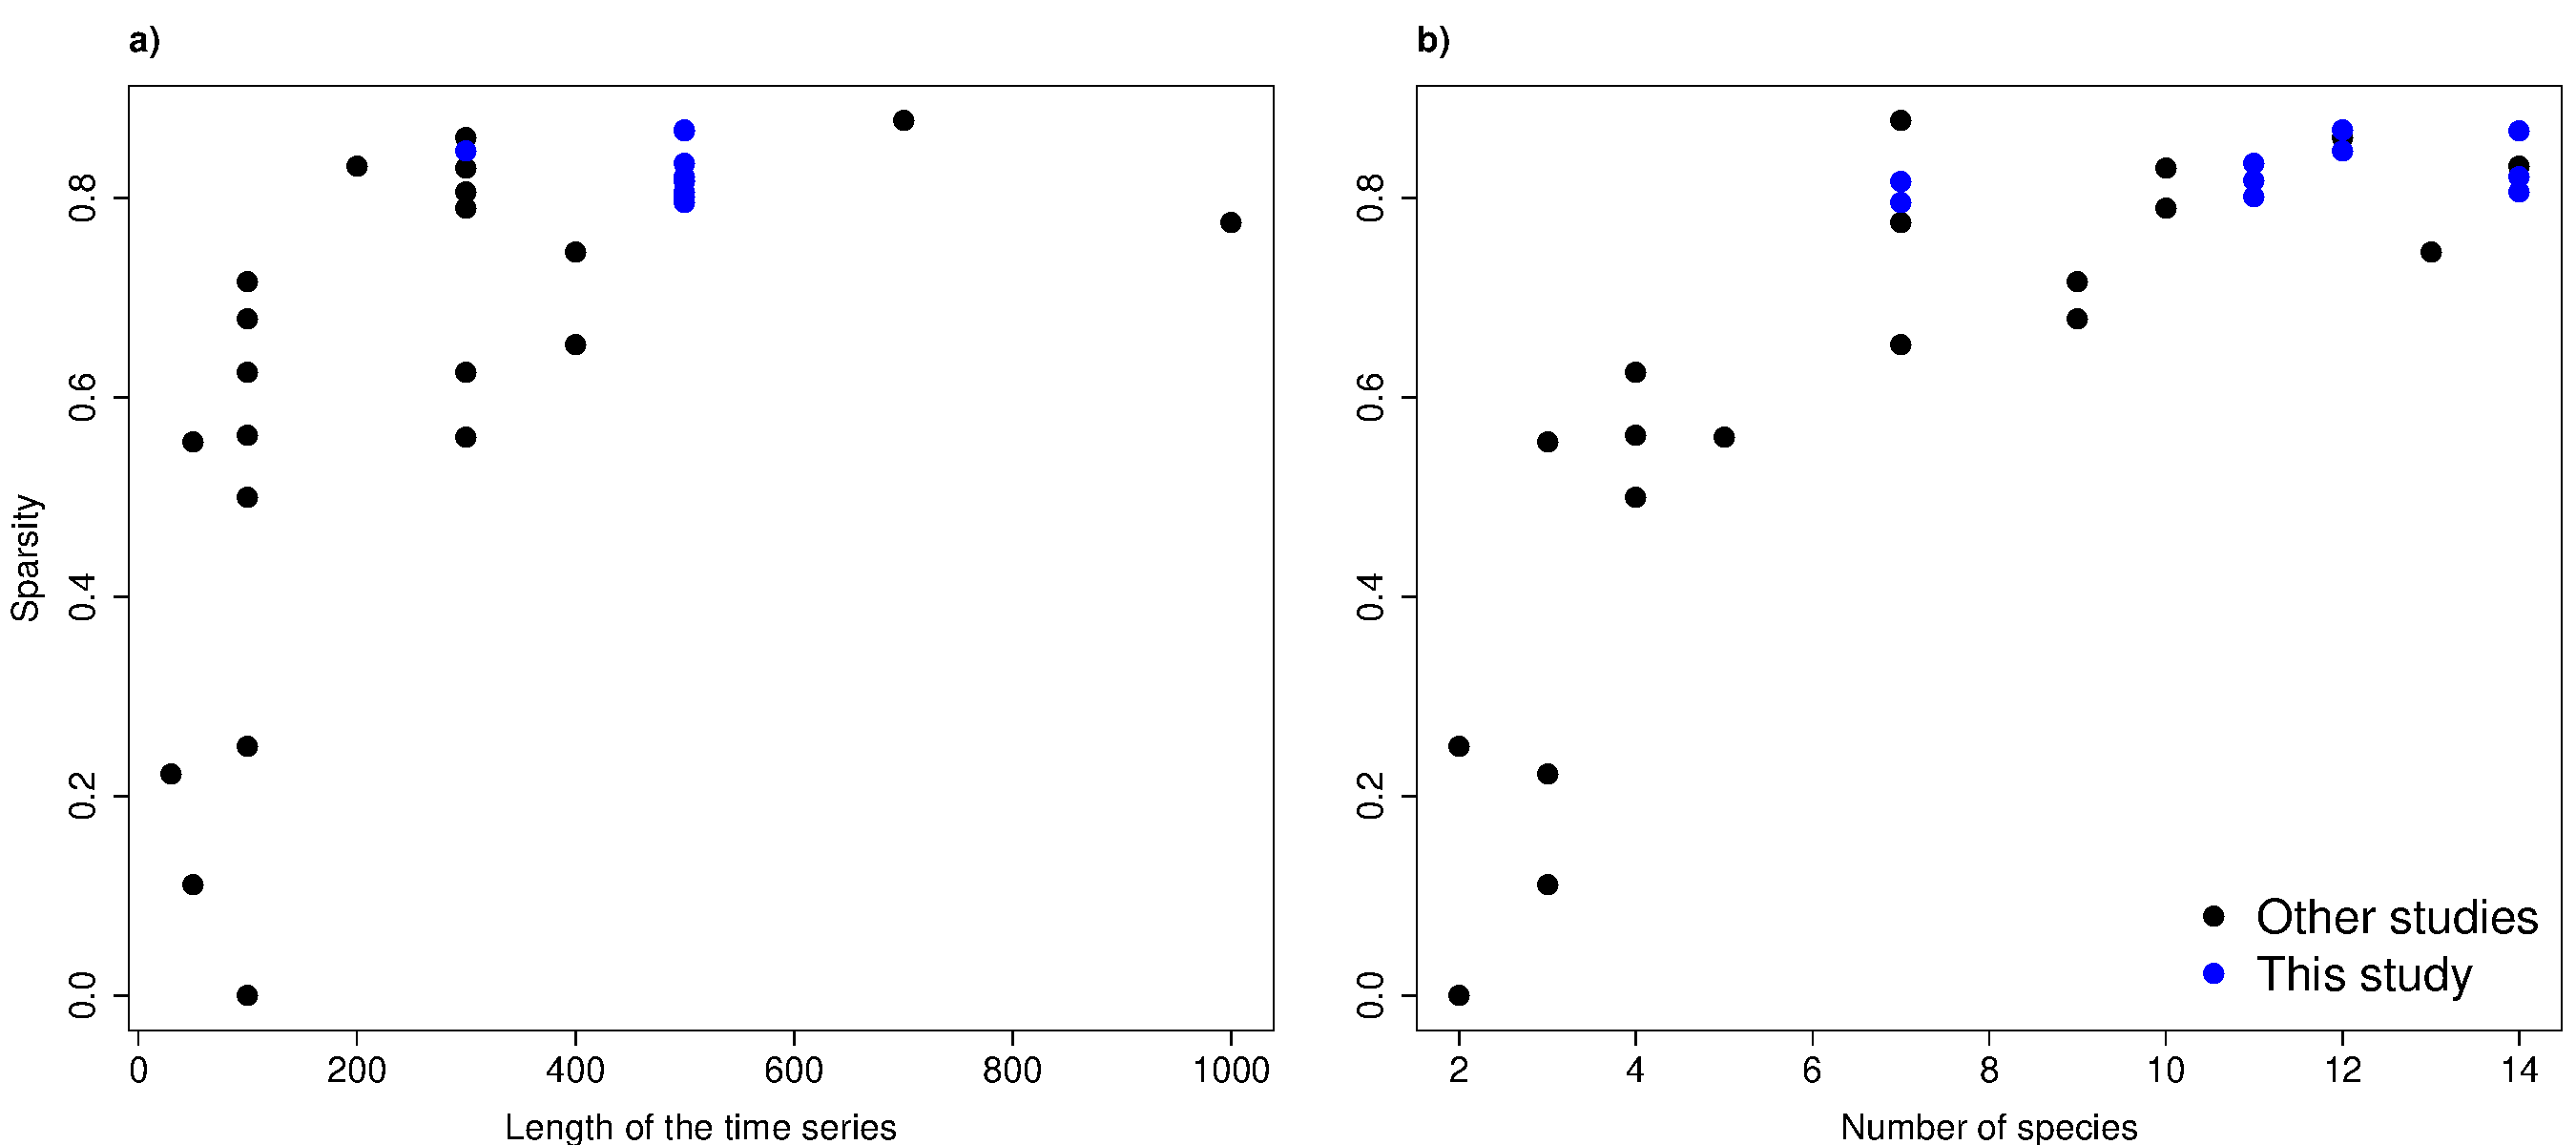
\includegraphics[width=0.8\textwidth]{graphe/sparsity_vs_others}
\par\end{centering}
\caption{\textbf{Relation between interaction sparsity and study design} in
studies described in Table \ref{tab:Studies}. Blue points correspond
to the present study. \label{fig:ratio_meta}\textit{ }}
\end{figure}

\printbibliography

\end{document}
